\documentclass[14pt]{extbook}
\usepackage{multicol, enumerate, enumitem, hyperref, color, soul, setspace, parskip, fancyhdr} %General Packages
\usepackage{amssymb, amsthm, amsmath, latexsym, units, mathtools} %Math Packages
\everymath{\displaystyle} %All math in Display Style
% Packages with additional options
\usepackage[headsep=0.5cm,headheight=12pt, left=1 in,right= 1 in,top= 1 in,bottom= 1 in]{geometry}
\usepackage[usenames,dvipsnames]{xcolor}
\usepackage{dashrule}  % Package to use the command below to create lines between items
\newcommand{\litem}[1]{\item#1\hspace*{-1cm}\rule{\textwidth}{0.4pt}}
\pagestyle{fancy}
\lhead{Progress Quiz 6}
\chead{}
\rhead{Version A}
\lfoot{9689-6866}
\cfoot{}
\rfoot{Spring 2021}
\begin{document}

\begin{enumerate}
\litem{
Solve the rational equation below. Then, choose the interval(s) that the solution(s) belongs to.\[ \frac{2x}{-4x -4} + \frac{-4x^{2}}{16x^{2} +24 x + 8} = \frac{4}{-4x -2} \]\begin{enumerate}[label=\Alph*.]
\item \( x_1 \in [-1.15, -0.74] \text{ and } x_2 \in [-1.4,0.7] \)
\item \( x \in [1.36,1.93] \)
\item \( \text{All solutions lead to invalid or complex values in the equation.} \)
\item \( x \in [-0.58,-0.05] \)
\item \( x_1 \in [-1.15, -0.74] \text{ and } x_2 \in [0.7,3.3] \)

\end{enumerate} }
\litem{
Determine the domain of the function below.\[ f(x) = \frac{6}{12x^{2} +21 x + 9} \]\begin{enumerate}[label=\Alph*.]
\item \( \text{All Real numbers.} \)
\item \( \text{All Real numbers except } x = a, \text{ where } a \in [-12, -12] \)
\item \( \text{All Real numbers except } x = a \text{ and } x = b, \text{ where } a \in [-1.04, -0.83] \text{ and } b \in [-0.88, -0.66] \)
\item \( \text{All Real numbers except } x = a \text{ and } x = b, \text{ where } a \in [-12, -12] \text{ and } b \in [-9.1, -8.84] \)
\item \( \text{All Real numbers except } x = a, \text{ where } a \in [-1.04, -0.83] \)

\end{enumerate} }
\litem{
Choose the graph of the equation below.\[ f(x) = \frac{1}{x + 2} - 3 \]\begin{enumerate}[label=\Alph*.]
\begin{multicols}{2}\item 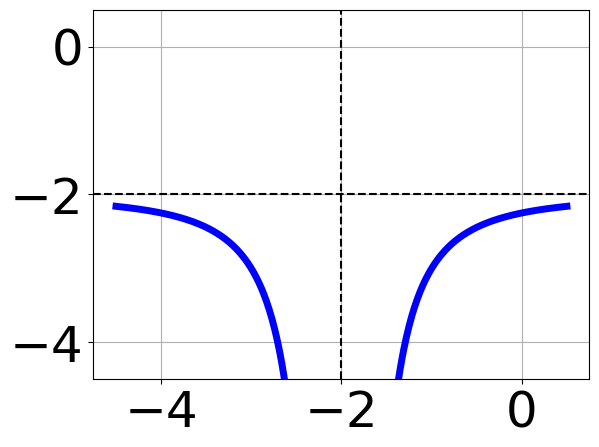
\includegraphics[width = 0.3\textwidth]{../Figures/rationalEquationToGraphAA.png}\item 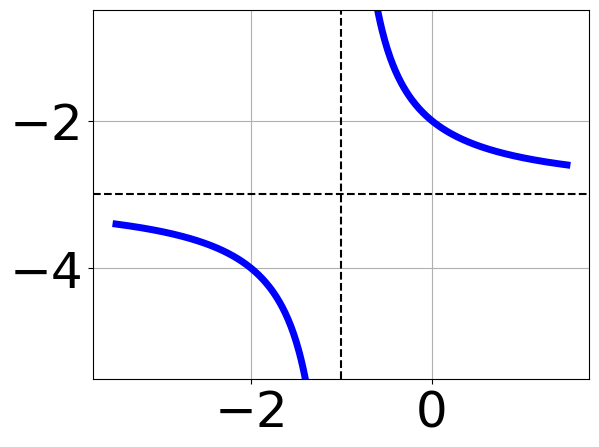
\includegraphics[width = 0.3\textwidth]{../Figures/rationalEquationToGraphBA.png}\item 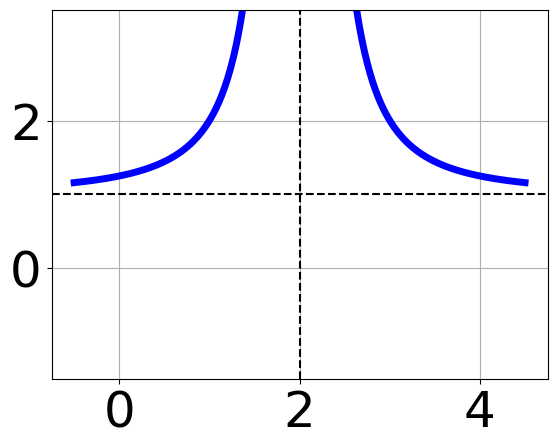
\includegraphics[width = 0.3\textwidth]{../Figures/rationalEquationToGraphCA.png}\item 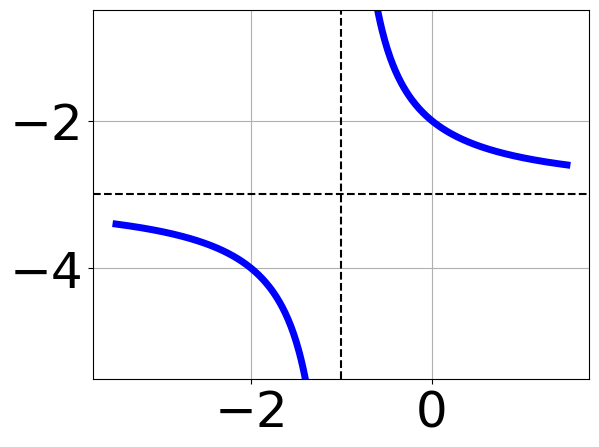
\includegraphics[width = 0.3\textwidth]{../Figures/rationalEquationToGraphDA.png}\end{multicols}\item None of the above.
\end{enumerate} }
\litem{
Choose the graph of the equation below.\[ f(x) = \frac{-1}{x + 2} - 3 \]\begin{enumerate}[label=\Alph*.]
\begin{multicols}{2}\item 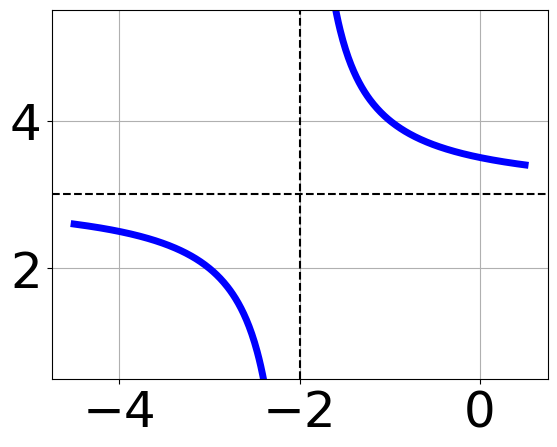
\includegraphics[width = 0.3\textwidth]{../Figures/rationalEquationToGraphCopyAA.png}\item 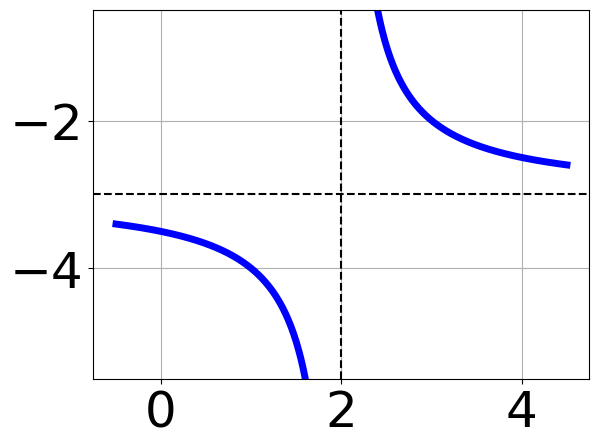
\includegraphics[width = 0.3\textwidth]{../Figures/rationalEquationToGraphCopyBA.png}\item 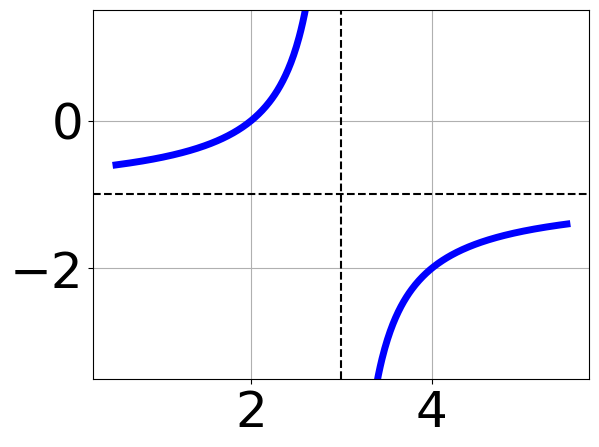
\includegraphics[width = 0.3\textwidth]{../Figures/rationalEquationToGraphCopyCA.png}\item 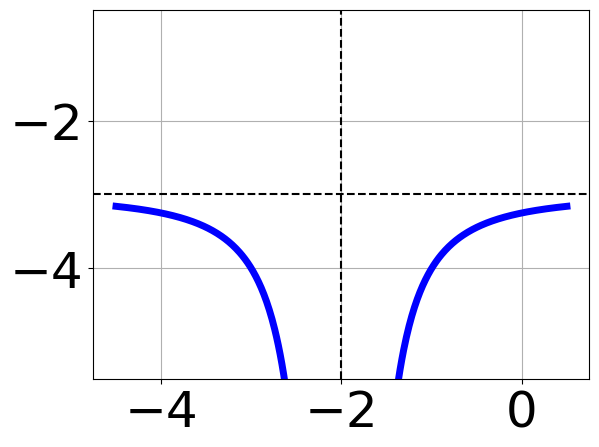
\includegraphics[width = 0.3\textwidth]{../Figures/rationalEquationToGraphCopyDA.png}\end{multicols}\item None of the above.
\end{enumerate} }
\litem{
Choose the equation of the function graphed below.
\begin{center}
    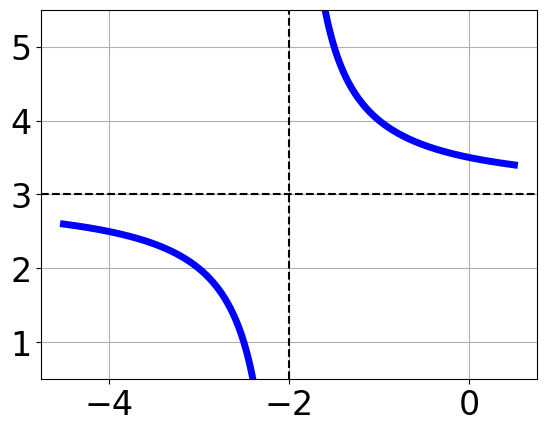
\includegraphics[width=0.5\textwidth]{../Figures/rationalGraphToEquationA.png}
\end{center}
\begin{enumerate}[label=\Alph*.]
\item \( f(x) = \frac{-1}{x - 2} + 2 \)
\item \( f(x) = \frac{1}{(x + 2)^2} + 2 \)
\item \( f(x) = \frac{1}{x + 2} + 2 \)
\item \( f(x) = \frac{-1}{(x - 2)^2} + 2 \)
\item \( \text{None of the above} \)

\end{enumerate} }
\litem{
Choose the equation of the function graphed below.
\begin{center}
    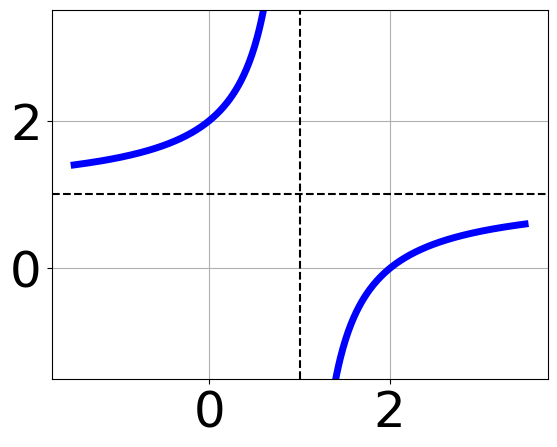
\includegraphics[width=0.5\textwidth]{../Figures/rationalGraphToEquationCopyA.png}
\end{center}
\begin{enumerate}[label=\Alph*.]
\item \( f(x) = \frac{-1}{x + 3} + 2 \)
\item \( f(x) = \frac{1}{(x - 3)^2} + 2 \)
\item \( f(x) = \frac{-1}{(x + 3)^2} + 2 \)
\item \( f(x) = \frac{1}{x - 3} + 2 \)
\item \( \text{None of the above} \)

\end{enumerate} }
\litem{
Solve the rational equation below. Then, choose the interval(s) that the solution(s) belongs to.\[ \frac{5}{-3x + 2} + 5 = \frac{-2}{18x -12} \]\begin{enumerate}[label=\Alph*.]
\item \( x_1 \in [0, 2] \text{ and } x_2 \in [1.02,1.19] \)
\item \( x_1 \in [-1.5, 0.8] \text{ and } x_2 \in [0.93,1.09] \)
\item \( x \in [0.98,1.98] \)
\item \( \text{All solutions lead to invalid or complex values in the equation.} \)
\item \( x \in [-1.5,0.8] \)

\end{enumerate} }
\litem{
Solve the rational equation below. Then, choose the interval(s) that the solution(s) belongs to.\[ \frac{-21}{28x + 35} + 1 = \frac{-21}{28x + 35} \]\begin{enumerate}[label=\Alph*.]
\item \( x_1 \in [-1.25, 0.75] \text{ and } x_2 \in [-3.25,-0.25] \)
\item \( x \in [-1.25,-0.25] \)
\item \( \text{All solutions lead to invalid or complex values in the equation.} \)
\item \( x \in [1.25,4.25] \)
\item \( x_1 \in [-1.25, 0.75] \text{ and } x_2 \in [0.25,2.25] \)

\end{enumerate} }
\litem{
Solve the rational equation below. Then, choose the interval(s) that the solution(s) belongs to.\[ \frac{-5x}{-3x -7} + \frac{-6x^{2}}{21x^{2} +55 x + 14} = \frac{-3}{-7x -2} \]\begin{enumerate}[label=\Alph*.]
\item \( x \in [-0.68,0.07] \)
\item \( x_1 \in [0.27, 1.06] \text{ and } x_2 \in [-4,-1.6] \)
\item \( \text{All solutions lead to invalid or complex values in the equation.} \)
\item \( x \in [-0.88,-0.63] \)
\item \( x_1 \in [0.27, 1.06] \text{ and } x_2 \in [-1.2,-0.8] \)

\end{enumerate} }
\litem{
Determine the domain of the function below.\[ f(x) = \frac{5}{36x^{2} +6 x -30} \]\begin{enumerate}[label=\Alph*.]
\item \( \text{All Real numbers except } x = a \text{ and } x = b, \text{ where } a \in [-36.1, -35.8] \text{ and } b \in [29.5, 30.3] \)
\item \( \text{All Real numbers except } x = a, \text{ where } a \in [-36.1, -35.8] \)
\item \( \text{All Real numbers except } x = a \text{ and } x = b, \text{ where } a \in [-1.3, -0.3] \text{ and } b \in [-0.3, 1.8] \)
\item \( \text{All Real numbers.} \)
\item \( \text{All Real numbers except } x = a, \text{ where } a \in [-1.3, -0.3] \)

\end{enumerate} }
\end{enumerate}

\end{document}